% !TEX root = Thesis.tex

%==============================================================================
\chapter{Towards Raman manipulation of spin-momentum state components}
\label{chap:raman_manipulation}
%==============================================================================

After the theoretical description of the Raman processes occurring in the diffraction of ultracold atomic ensembles, the following step consists in the generation of momentum and spin states components. The process has a strong resemblance with the previously described, with the added factor that now every momentum state also carries a different internal energy state. This is due to Raman transitions taking place inside the Zeeman levels that erbium's ground state was split into. For the experimental process to function as expected, it is required a given magnetic field $\vec{B}_\text{R} = B_{\text{R}} \vec{e}_x$ along the optical lattice axis $x$. This field will produce the Zeeman splitting of the ground state, and the optical lattice will be in charge of producing the Raman transitions, separating the atomic ensemble into multiple energy levels. However, two photon detuning condition must be fulfilled for this process to happen, and now it corresponds with the energy difference between two Zeeman split states $\Delta E_\text{R} = g_J \mu_B B_\text{R}$ \cite{Foot2005}. Due to this, knowing the exact value of $\Delta E_\text{R}$ becomes a key factor, and any background magnetic fields  affecting the \ac{bec} can produce values for the Zeeman splitting very different to the expectation. For this reason, a preparatory experiment must be carried out, that allows the estimation of $\Delta E_\text{R}$ and helps with the compensation of background fields in favour of the known $\vec{B}_\text{R}$ field.

\section{\Acl{rf} transitions and the Stern-Gerlach experiment}

The objective of this experiment is to quantify the Zeeman splitting induced into an erbium \ac{bec}. As it can be seen in Figure \ref{fig:erbium_scheme}, the energetic ground state of erbium has a total electronic angular momentum of $J = 6$. When the atomic ensemble is being affect by a magnetic field $\vec{B}_\text{H}$, the ground state gets Zeeman split into $2J+1 = 13$ energy states with the secondary quantum number $m_J = \text{-6, -5, ..., +6}$, each state with energy \cite{Foot2005}
\begin{equation}
	E_\text{Ze} = g_J \mu_B m_J B_\text{H}
\end{equation}

Where $g_J$ represents the Landé g-factor and for this case it is $g_J\approx11/6$. Due to the way in which the experimental set-up is constructed, the \ac{mot}'s \SI{583}{\nano\meter} beam light that interacts with erbium in the $z$ axis, by pushing the atoms against gravity, is $\sigma^-$ polarized \cite{Ulitzsch2016}. Due to the fact that this beam interacts mostly with the atomic ensemble, it forces the atoms to remain the energetic state with $m_J = -6$. This prevents the direct splitting of the erbium \ac{bec} into different orders by regarding energetic differences. To allow for transitions between these different Zeeman states, the atomic ensemble must interact with a \acf{rf} pulse. Moreover, in order to distinguish which orders the \ac{rf}-pulse has transitioned the atomic ensemble into, a Stern-Gerlach experiment must be performed. This consists in the use of a magnetic inhomogeneous field $B_\text{IH}(\vec{r})$ that separates the atomic \ac{bec} spatially according the quantum number $m_J$. The force that allows this is commonly called Stern-Gerlach force and is due to the non-zero gradient applied to the Zeeman term in the hamiltonian \cite{Foot2005}
\begin{equation}
	\vec{F}_\text{SG}(\vec{r}) = \grad{(\vec{\mu}\cdot\vec{B}_\text{IH}(\vec{r}))}
\end{equation}

Where $\vec{\mu}$ represents the atomic magnetic moment. Therefore, for $B_\text{IH}(\vec{r})$ pointing in any arbitrary $z$ direction, the force applied to the different $2J+1$ levels can be obtained as
\begin{equation}\label{eq:Stern-Gerlach_force}
	\vec{F}_\text{SG}(\vec{r}) = - g_J \mu_B m_J \frac{\partial B_\text{IH}(\vec{r})}{\partial z}
\end{equation}

Which is $m_J$ dependant and produces, as a result, different contributions to the energetic states. This kind of force will make possible the separation of a \ac{bec} in Zeeman orders, and the analysis of internal energetic behaviour after the interaction with a given \ac{rf}-pulse. The use of both these tools permits the creation of an experimental set-up that can quantify the energetic difference between contiguous Zeeman orders
\begin{equation}\label{eq:Zeeman_splitting_difference}
\Delta E_\text{Ze} = g_J \mu_B B_\text{H}
\end{equation}

For a given spatially homogeneous field $\vec{B}_\text{H}$, interacting initially with an atomic ensemble. The experimental procedure can be described as follows:
\begin{itemize}
	\item First, there is a change in the magnetic field $\vec{B}_\text{H}$ acting on the atomic \ac{bec} during its final formation process, the last \SI{10}{\milli\second} of the evaporation cooling phase. This allows to change in different experiment cycles the homogeneous magnetic field $\vec{B}_\text{H}$ and therefore, the Zeeman splitting of the \ac{bec} ground energy level, given by $\Delta E_\text{Ze}$ in Equation \eqref{eq:Zeeman_splitting_difference}.
	\item Then, \SI{2}{\milli\second} after the evaporation phase, the \ac{rf}-pulse is used while $\vec{B}_\text{H}$ is kept unchanged. This \ac{rf}-pulse has a given duration $t_\text{RF}$, an intensity $I_\text{RF}$ and a frequency $\nu_\text{RF}$. As a result, the erbium \ac{bec} transitions between the initial state $m_J=-6$ to the rest of states, when $\nu_\text{RF}\approx\frac{\Delta E_\text{Ze}}{\hbar}$ the resonant frequency for the Zeeman transition. Moreover, due to the fact that these transitions also result in Rabi oscillations, the magnitudes $t_\text{RF}$ and $I_\text{RF}$ must be adjusted to produce $\frac{\pi}{2}$ pulses and favour the atomic transitions into the rest of Zeeman states.
	\item Finally, after the atomic \ac{bec} interaction with the \ac{rf}-pulse, the ensemble falls due to gravity during a \acl{tof} $t_\text{TOF}$. In this time period, the magnetic field gradient $B_\text{IH}(\vec{r})$ is activated and the atomic \ac{bec} receives a state dependant Stern-Gerlach force given by Equation \eqref{eq:Stern-Gerlach_force}. This results in the spacial separation of the Zeeman levels after the \ac{tof}, which can be imaged by the absorption imaging phase.
\end{itemize}

As a result, the experiment allows to measure the resulting orders after a \ac{rf}-\ac{bec} interaction. By varying $\nu_\text{RF}$, one can make a measurement of the resonant frequency to the Zeeman splitting produced by any homogeneous field $\vec{B}_\text{H}$. In addition to the transition's line-width estimation, which is a parameter deeply related to the stability of $\vec{B}_\text{H}$ during the interaction time $t_\text{RF}$. To conclude, the experiment allows to measure the Zeeman splitting of any given field $\vec{B}_\text{H}$, compensate for the effect $\Delta E_\text{Ze}\approx0$ by changing $\vec{B}_\text{H}\rightarrow \vec{B}_\text{Comp}$, and also permits to add any wished field $\vec{B}_\text{H} = \vec{B}_\text{Comp} + B_{\text{R}} \vec{e}_x$ in the desired lattice $x$ direction, which results in $\Delta E_\text{Ze}\approx\Delta E_\text{R}$ the Zeeman splitting between orders in the $x$ axis. Resulting in a fairly good estimation of $\Delta E_\text{R}$ due to $\vec{B_{\text{R}}}$, which will give the two photon detuning condition for Raman manipulation in the following section. This procedure and the experimental set-up have been described in more detail here \cite{Ulitzsch2016}.

\section{Raman manipulation of spin-momentum state components}

\begin{figure}[!htbp]\centering
	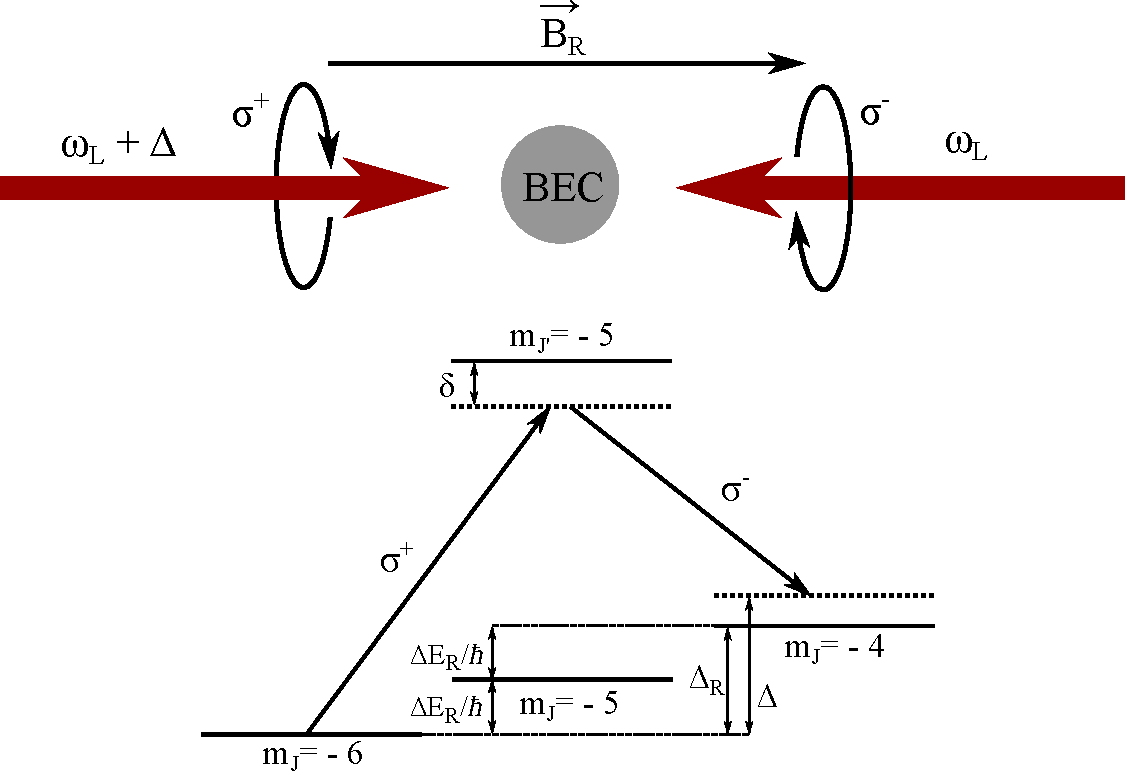
\includegraphics[width=0.8\columnwidth]{rama_spin_mainpulation.pdf}
	\caption[Experimental and energetic scheme of the 2-photon Raman transition process in the spin-momentum configuration]{Experimental and energetic scheme of the 2-photon Raman transition process in the spin-momentum configuration. In this case, the optical scheme is very similar to the described in Chapter \ref{chap:one_dimensional_lattices} with the addition of a magnetic field $\vec{B}_\text{R}$ in the lattice direction $x$ and the circular polarization $\sigma^\pm$ of both beams forming the lattice. Moreover, the energetic scheme also relates to the Raman process described in Chapter \ref{chap:one_dimensional_lattices}, with the only difference that now the two photon detuning condition becomes the so-called Raman condition given by $\Delta_\text{R} \equiv 2\Delta E_\text{R}/\hbar$. As a result, the orders generated in the Raman process not only have different momentum components but also spin values  $m_\text{J}=-6 \rightarrow m_\text{J}=-5$, which means internal energetic differences in the generated orders. }\label{fig:raman_manipulation}
\end{figure}

%%% Local Variables: 
%%% mode: latex
%%% TeX-master: "Thesis"
%%% End: 
